\documentclass[12pt]{article}
\usepackage[english]{babel}
\usepackage[T1]{fontenc}
\usepackage[utf8]{inputenc} % or \usepackage[utf8x]{inputenc} for more characters
\usepackage{eurosym}
\usepackage{textcomp}
\usepackage{afterpage}
\usepackage{hyperref}
\usepackage{xcolor}
\usepackage{listings}
\usepackage{xparse}
\NewDocumentCommand{\codeword}{v}{%
\texttt{\textcolor{blue}{#1}}%
}
\lstset{language=java,keywordstyle={\bfseries}}
\usepackage{amsfonts}
\usepackage{amsmath}
\usepackage{amsthm}
\usepackage[left=3cm, right=3cm, top=3.5cm, bottom=3.5cm]{geometry}
\usepackage{mathabx}
\lstset{
   basicstyle=\fontsize{9}{10}\selectfont\ttfamily
}
\newcommand\blankpage{%
    \null
    \thispagestyle{empty}%
    \addtocounter{page}{-1}%
    \newpage}

\usepackage{graphicx}

\usepackage{sectsty}
\usepackage[explicit]{titlesec}

\newtheorem{theorem}{Theorem}

\allsectionsfont{\raggedright}


\begin{document}


\begin{titlepage}

\begin{center}

UNIVERSITY OF "ALEXANDRU IOAN CUZA" IAȘI
\\
\textbf{Faculty of Computer Science}
\end{center}

   \vspace{20mm}

\begin{center}
    \includegraphics{figures/fii.png}
\end{center}
   \vspace{10mm}
\begin{center}
	\Large{BACHELOR'S THESIS}\\
	
	\vspace{10mm}
	
	\large \textbf{Extenstion to the Key-Policy Attribute Based Encryption schema}\\
	\vspace{5mm}
	
	proposed by
	
	\vspace{5mm}
	\large\textit {LUCA ANDREI}
	\\
	\vspace{20mm}
	\textbf{Date: }\textit{july, 2018}\\
	\vspace{10mm}
	\textbf{Coordinator}\\
	\textbf{\textit{Prof.dr. Țiplea Ferucio Laurențiu}}
	\vspace{30mm}
\end{center}
\end{titlepage} 

\afterpage{\blankpage}

\onecolumn
\tableofcontents
\twocolumn

\onecolumn

\section{Introduction}

\subsection{Overview}

The \textit{Attribute based Encryption} field has been growing during the past years, but still lots of its problems  remain unsolved, for example the \textit{Key-Policy Attribute based Encryption} proposed in \cite{gpsw} was successfully attacked using the \textbf{Backtracking attack} proposed in \cite{gghsw}. The same paper proposed a new schema to solve this problem based on multilinear maps, but this causes problems on the actual implementation of the schema, because at his moment, we don't have a proper way of generating these multilinear maps that preserves the security correctness. In this context, \cite{fltccd} paper proposed a new \textit{Key-Policy Attribute based Encryption} schema based on bilinear maps that thwarts the \textbf{Backtracking attack} but introduces another level of complixity by using \textbf{FO(Fan-Out) gates} for the boolean circuits. 

This paper introduces an extension and the first implementation of the schema proposed in \cite{fltccd}. First of all, the extension puts forward a new way of defining the boolean circuits used for key construction by using threshold gates providing this way a more flexible construction of the boolean circuits. Second of all, the implementation is made in Java and uses the \textbf{Java Pairing-Based Cryptography Library} that provides an implementation of bilinear maps and operations on its elements and the \textbf{Bouncy Castle Library} for defining the cryptographic structures.

\vspace{80mm}

\subsection{Related work}

This section is divided in two sections that show a part of the related works(or papers) with the extension of the \textit{threshold gates} in the \cite{fltccd} schema and specifies some preceding implementations from which this paper has inspired.  

\subsubsection{Extension}

The extension of the boolean circuits proposed in \cite{fltccd} schema by using threshold gates is obviously based on the \cite{fltccd} paper that proposes the first \textit{Key-policy Attribute-based Encryption (KP-ABE) scheme for monotone Boolean circuits based on bilinear maps}. This schema is an extension of the schema proposed in \cite{gpsw} and it uses just one bilinear map and secret sharing procedures. The problem with the schema mentioned in \cite{gpsw} is that it can be attacked using the \textbf{Backtracking attack} that we'll discuss on the \textit{Preliminaries} section. 

As mentioned in \textit{Overview}, there is another schema based on multilinear maps proposed in \cite{gghsw} that solves this problem but seems to be complicated to put this into practice because the current model of multilinear maps(see \cite{ggh}) was proven that can be broken using the \textbf{Annihilation attacks} proposed in \cite{msz}. Until another multilinear maps valid candidate implementation is proposed, using multilinear maps can cause problems and currently are unsafe.

Even though the \cite{fltccd} schema uses just one bilinear map it is more efficient than the one in \cite{gghsw} if the boolean circuits do not have Fan-Out gates connected between them by paths. These Fan-Out gates are needed to make this schema resistant to the \textbf{Backtracking attack}. As result, during the \textit{share} procedure, the key components can be increase exponentially based on the number of the chained Fan-Out gates.

Other related works that were used for this paper writing were based on the \textbf{Secret Share Schemas(SSS)} because when using the \textit{threshold gates - (k, N)} it is needed to divide some key information \textit{I} in \textit{N} pieces and allow it to be reconstructed \textit{if and only if} at least \textit{k} pieces of shared information are knowed. This problem have lived for a long time and it has a solution based on \textbf{Lagrange interpolation} proposed by \textit{Adi Shamir} in \cite{shamir} that we inspired from also in this paper. Another secret sharing schemes proposed were by \textit{Blakley} in \cite{blakley}, by \textit{Brickell} in \cite{brickell} and by \textit{M. Ito, A. Saito, and T. Nishizeki} in \cite{isn}.

\subsubsection{Implementation}

The implementation related works are based on the \textbf{Pairing-Based Cryptography(PBC) Library}\cite{pbc} that is a C library based on the GMP library\cite{gmp}. What this paper uses though is the \textbf{Java Pairing-Based Cryptography(jPBC) Library}\cite{jpbc} that provides a wrapper over the \textbf{PBC} library. 

The current implementations(related to ABE) that the author of the \textbf{jPBC} library provides are for the \textit{Attribute-Based Encryption for Circuits from Multilinear Maps}\cite{gghsw} schema and for the \textit{How to Compress (Reusable) Garbled Circuits}\cite{gghvv} model. These implementations were the starting point for the implementation proposed in this paper and we tried to preserve the general structure of the implementation according to schemas already implemented(defined using \textit{Bouncy Castle Library}\cite{bc}).

\section{Preliminaries}

In this section we'll be talking about the terminology and the notations used by this paper and also, where is the case, we'll describe the primitives that can be used with the \textbf{jPBC} library to perform some of these operations.  

\subsection{Identity based Cryptography}

The \textit{Identity based Cryptography} represents an extension of the classic \textit{public-key cryptography} where the public-key is represented by some distinctive public information like the email address, phone number or some personal identification number.

This paradigm was first proposed by \textbf{Adi Shamir} in \cite{shamirid}(1984) and it took sixteen years until it found its first implementations in \cite{sok}(2000) and \cite{bf}(2001). This delay was caused by the need of having a private key generator entity that manages the actual public/private key pairs in the system. 

\subsection{Attribute based Encryption}

The \textit{Attribute based Encryption} is a relatively recent way of thinking about cryptograpy that has its roots in \textit{asymmetric cryptography} and in \textit{identity criptography}. Basically what this idea brings forward is that instead of having a \textbf{private key} that authenthicates a specific user(in public key systems) or an \textbf{email}(for example in identity based systems) you're having a set \textit{A} of attributes(ex: the country he lives on, the birthplace, workplace) from a universal set of attributes $U$ that can allow you to access the resources of a system. 

This paradigm is especially suited in access control systems like \textit{operating systems} or \textit{Cloud access management systems}(see: IAM services from Amazon Web Services or Google Cloud) where every entity in that system is given a the set of attributes that we've been talking above and using them with \textit{boolean circuits}(see the below section for more details) for defining the rules of the access control system it generates the encryption/decryption key needed for the resources of the system.  

Currently there are two ways of using the Attribute based Encryption: the \textit{Key-Policy Attribute based Encryption}(KP-ABE) and \textit{Cipher-Policy Attribute based Encryption} that we'll detail in the next section. Both of these policies use boolean circuits for defining the access structure based on the attributes and the difference comes from the way they decide to make use of the access structure (one uses the structure at the encryption phase and the other one at decryption phase).

\subsubsection{General Attribute based Encryption schema structure}

\begin{itemize}
	\item Setup
		\begin{itemize}
			\item Input: a security parameter $S$
			\item Output: a public key/parameters $PP$ that is used for the encryption phase and secret master key of the system $MSK$ that is used for the secret key generation
		\end{itemize}
	\item Encryption
		\begin{itemize}
			\item Input: the resource $R$ that is encrypted, the public key/parameters $PP$ and set of attributes $A$ for encryption (for \textit{KP-ABE}) or the access structure $AS$(for \textit{CP-ABE})
			\item Output: the encrypted resource $E$
		\end{itemize}
	\item Key Generation
		\begin{itemize}
			\item Input: the master key $MK$ and the access structure $AS$ of the user (for \textit{KP-ABE}) or the set of attributes $A$ of the user (for \textit{CP-ABE}) 
			\item Output: the secrey key $SK$(information associated with the attributes)
		\end{itemize}
	\item Decryption
		\begin{itemize}
			\item Input: the encrypted resource $R$, the secret key $SK$ and the access structure $AS$
			\item Output: the plain(unencrypted) resource if the $AS$ matches with the values provided with the $SK$ or an error otherwise
		\end{itemize}
\end{itemize}

\subsection{Key-Policy and Cipher-Policy Attribute based Encryption}

\begin{itemize}
  \item \textit{Key-Policy Attribute based Encryption} is the policy addressed in the \cite{fltccd} and since we're making an extension of this schema, this will be the policy that we're covering in this paper. The KP-ABE is the policy that in the \textit{encryption} phase takes as input a resource, some security parameters generated by the \textit{setup} phase and the attributes used for the encryption. Then, in the \textit{key generation}/\textit{decryption} phases, the user takes his own access structure and attributes and tries to generate the decrpytion key of the resource. If his access structure and the attributes need for the decryption of the resource match, then the user can generate the decryption key and access it, if the attributes are not sufficient or the access structure doesn't permit access based on the attributes, the user cannot generate the decrpytion key (see \textit{Figure 1}).

  \begin{center}
  	\begin{figure}[htpb]
    \centering
    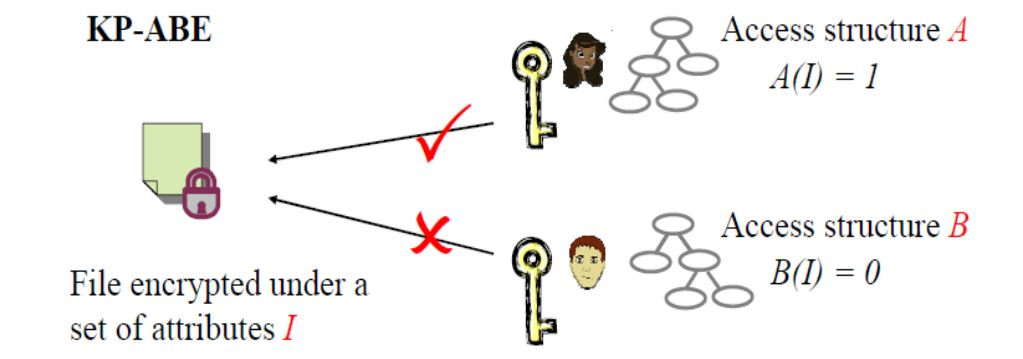
\includegraphics[width=\textwidth,height=5cm,keepaspectratio=true]{figures/KP-ABE.JPG}
    \caption{
        Key-Policy Attribute based Encryption visual representation from \cite{ka}
    }
	\end{figure}
  \end{center}

  \item \textit{Cipher-Policy Attribute based Encryption} is a policy that appeared after the classical KP-ABE but it is simpler and more natural than the previous construction that is more suited for complex access structures. This policy takes in the \textit{encryption} phase a access structure and the resource that needs to be encrypted (notice that the KP-ABE takes as input the attributes) and the security parameters given by the \textit{setup} phase. Then, in the \textit{key generation}/\textit{decryption} phases, the user takes his attributes and uses them with the access structure of the resource in order to gain access: if his attributes and the resource structure match, he can generate the decryption key and thus he gains access to that resource, otherwise the access is denied (he cannot generate the decryption key - see \textit{Figure 2}).

  \begin{center}
  	\begin{figure}[htpb]
    \centering
    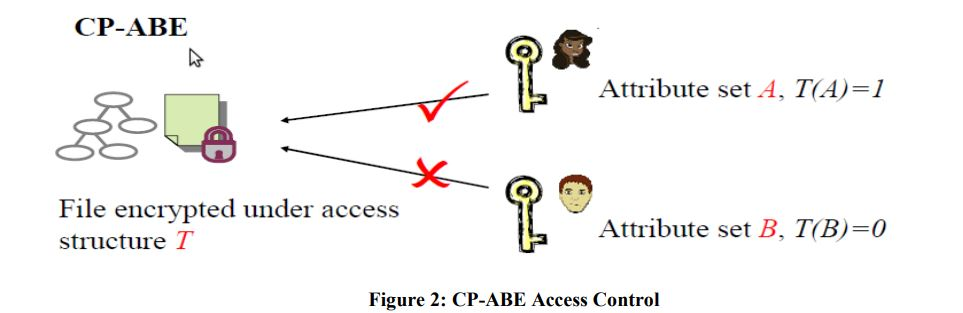
\includegraphics[width=\textwidth,height=5cm,keepaspectratio=true]{figures/CP-ABE.JPG}
    \caption{
        Cipher-Policy Attribute based Encryption visual representation from \cite{ka}
    }
	\end{figure}
  \end{center}
\end{itemize}

\subsection{Bilinear maps}

Let $G_1$ and $G_2$ two multiplicative cyclic groups of prime order $p$ and a function $e : G_1 \times G_1 \leftarrow G_2$. The function $e$ is called bilinear map if:

$$e(x^a, y^b) = e(x, y)^{ab}, \forall x, y \in G_1 \textrm{ and } a, b \in \mathbb{Z}_p \textrm{ and,}$$

$$e(g, g) \textrm{ is a generator of } G_2, \forall g \textrm{ generator of } G_1$$

The \textbf{jPBC} library provides costruction of bilinear maps from eliptic curves by specifing the type of curve that you intend to use. It has support for different types of curves like $A$ curves($y^2 = x^3 + x$), curves based on \textit{Diophantine} equation, etc.. The class that represents a bilinear map is called \textit{Pairing} in \textbf{jPBC} and you can instatiate this class using the following (example for $A$ type curve):

\begin{lstlisting}
PairingFactory.getPairing(new TypeACurveGenerator(rBits, qBits)
			  .generate())
\end{lstlisting} 

where the rBits and qBits are the curve parameters. For other curves the parameters may be different, but the idea is that you can use the \textit{PairingFactory} class to generate the desired bilinear map. You can also specify in a file other types of bilinear maps derived from the \textbf{PBC} library and currently there are not known any compatibility issues.

To apply a bilinear map to some given elements of $G_1$, $element_1, element_2$ you can achive that by using the following code:

\begin{lstlisting}
Element result = pairing.pairing(element1, element2);
\end{lstlisting} 

Some other useful operations might be:

\begin{lstlisting}
// get the Z_r field object
Field zr = pairing.getZr();

// get G_1 field object
Field g1 = pairing.getG1();

// new random element from Z_r
Element e1 = zr.newRandomElement();

// new identity element of Z_r
Element e2 = zr.newOneElement();

// new zero element of Z_r
Element e3 = zr.newZeroElement();

// addition, multiplication, pow
e1.add(e2);
e1.mul(e2);
e1.powZn(e2);
\end{lstlisting} 

\subsection{Decisional Bilinear Diffie-Hellman assumption}

Let $G_2$ be a bilinear group of order $p$ and $g$ a generator of this group. The \textit{Decisional Bilinear Diffie-Hellman assumption}(DBDH assumption) states that given $g^a, g^b, g^c, g^z$ where $a, b, c, z \in \mathbb{Z}_p$ randomly chosen and $g$ is the generator of group $G_1$, you can't distinguish from $e(g, g)^{abc}$ and $e(g, g)^z$ using a \textit{probabilistic polynomial-time} algorithm for the elements of $G_2$.

We'll use the \textit{DBDH assumption} for the security proof our extension.

\subsection{Boolean circuits}

A \textbf{boolean circuit} is a mathematical model that represents tree (binary in its classic form) where the leaf nodes are considered input values (\textit{boolean values} - \textit{true} or \textit{false}), the internal nodes represent boolean functions like \textit{OR, AND, NOT}. To evaluate this tree, one has to give the values to the input nodes and then traverse bottom-up the tree and for each node, look at its children values, apply the function defined for that node and update the circuit with its result. 

In this paper we'll focus on \textit{monotone boolean circuits} that means that thea are not allowed \textit{NOT} gates, but that does not consitute a loss of generality (see \cite{gghsw}). Also, the gates used in this paper have the following restricion: all the input gates have exactly one output wire (fan-out one), this is not a limitation because as proposed in \cite{fltccd} there can be used the \textit{Fan-Out gates} to achive a fan-outs greater than one for any gate (inclsively input gates). The FO-gates are a special type of gates with exactly one input and can have any number of outputs (any fan-out number) and what are these gates doing is that propagates the input values to the output values.

\subsubsection{Threshold gates}

The \textit{Threshold gates} come as an extension of the usual \textit{boolean circuits} gates $OR$ and $AND$ gates. A $(k, N)$ threshold gate represent a logical gate that have as input N values and in order to be evaluated as $true$ it has to have at least $k$ values from the input evaluated as $true$, otherwise the result of this gate is evaluated as $false$. For example, a $OR$ gate can be viewed as a $(1, 2)$ gate and a $AND$ gate can be viewed as a $(2, 2)$ gate.

\subsubsection{Example}

For the \textit{boolean circuit} in \textit{Figure 3} if the input of the gates is $[false, false, true, true]$, then result of the circuit will be $true$ because the gate $6^{th}$\textit{ gate(AND)} gate will be evaluated as $true$ and then the $8^{th}$\textit{ gate (OR)} gate will also be $true$.

If the input is $[true, false, false, true]$ the result of the circuit will be $false$ because the  $5^{th}$\textit{ gate (OR)} is evaluated as $false$, the $6^{th}$\textit{ gate (AND)} is evaluated with $false$, the $7^{th}$\textit{ gate (AND)} is evaluated as $false$ and as result the $8^{th}$\textit{ gate (OR)} will be evaluated with $false$.

\begin{center}
	\begin{figure}[htpb]
\centering
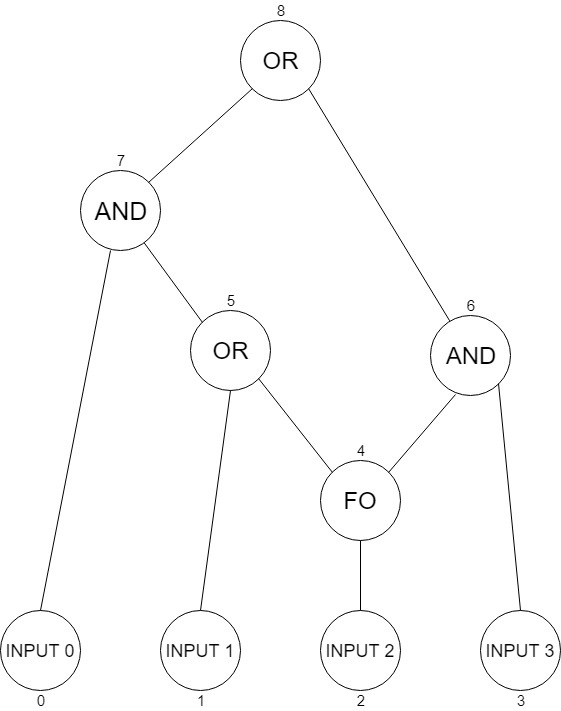
\includegraphics[width=\textwidth,height=8cm,keepaspectratio=true]{figures/boolean-circuit-fltccd.jpg}
\caption{
    Boolean circuit exmple that was also proposed in \cite{fltccd}
}
\end{figure}
\end{center}

The code that generates the boolean circuit above where $n$ is the number of inputs and $q$ is the number of internal gates:

\begin{lstlisting}
// regular gates
circuit = new DefaultCircuit(n, q, 3, new DefaultGate[]{
        new DefaultGate(INPUT, 0, 1),
        new DefaultGate(INPUT, 1, 1),
        new DefaultGate(INPUT, 2, 1),
        new DefaultGate(INPUT, 3, 1),

        new DefaultGate(FO, 4, 2, new int[]{2}),
        new DefaultGate(OR, 5, 3, new int[]{1, 4}),
        new DefaultGate(AND, 6, 3, new int[]{3, 4}),
        new DefaultGate(AND, 7, 4, new int[]{0, 5}),
        new DefaultGate(OR, 8, 3, new int[]{6, 7})
});

// threshold gates
circuit = new DefaultCircuit(n, q, 3, new DefaultGate[]{
        new DefaultGate(INPUT, 0, 1),
        new DefaultGate(INPUT, 1, 1),
        new DefaultGate(INPUT, 2, 1),
        new DefaultGate(INPUT, 3, 1),

        new DefaultGate(FO, 4, 2, new int[]{2}),
        new DefaultGate(KN, 5, 3, new int[]{1, 4}, 1),
        new DefaultGate(KN, 6, 3, new int[]{3, 4}, 2),
        new DefaultGate(KN, 7, 4, new int[]{0, 5}, 2),
        new DefaultGate(KN, 8, 3, new int[]{6, 7}, 1)
});
\end{lstlisting} 

\subsection{The Backtracking Attack}

The \textit{Backtracking Attack} was first proposed in \cite{gghsw} and it is the reason why the \cite{gpsw} schema is not applicable to monotone boolean circuits that have a fanout greater than one. In the \cite{gghsw} it was proven that by using an unathorized set of input attributes for a access structure you can generate the decryption key by exploiting the way that the schema uses the \textit{OR} gates for the \textit{key generation} phase.

The problem comes from the fact that in the \textit{key-generation} phase (that is executed top-down) the output value of a \textit{OR} gate $G$ is propagated to both of its inputs unchanged. In the \textit{decryption} phase (that is executed bottom-up) it check if the inputs of $G$ are defined and if at least one of them is defined, then the decryptor also knows the other input's value and if that other gate has a fan out greater than one, it can be used to gain access using an unauthorized set of attributes.

\subsubsection{Example}

In this section we'll show how the \textit{share} and \textit{reconstruction} phases work for \textit{OR} gates and how the \textit{Backtracking attack} takes advatage of this construction for the gates that have a fan out greater than one.

In \textit{Figure 4} is shown that for a \textit{OR} gate, the \textit{share} phase (the boolean circuit is traversed top-down) leaves the output value of the gate unchanged and propagates it to the inputs. 

\begin{center}
	\begin{figure}[htpb]
\centering
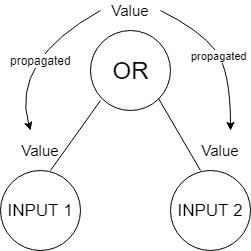
\includegraphics[width=\textwidth,height=4cm,keepaspectratio=true]{figures/shareOR.jpg}
\caption{
	The share procedure for a OR gate.
}
\end{figure}
\end{center}

In \textit{Figure 5} it is shown the \textit{reconstruction} (the boolean circuit is traversed bottom-up) procedure for a \textit{OR} gate. In this example, the authorized attribute (or the user has attribute associated with this gate) is the \textit{INPUT 1} while the \textit{INPUT 2} is unauthorized (or the user does not have that attribute/secret). The \textit{reconstruction} phase looks if at least one of its input value is known, in our example the value of \textit{INPUT 1} is known and then propagates this value to the output of the \textit{OR} gate. From the way that the \textit{share} procedure is constructed for the \textit{OR} gate, it is sure that the other value of the input must be the same as the value of the \textit{INPUT 1}, thus an attacker can discover the value of the attribute associated with \textit{INPUT 2}.

\begin{center}
	\begin{figure}[htpb]
\centering
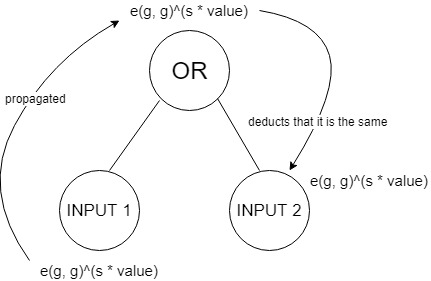
\includegraphics[width=\textwidth,height=5cm,keepaspectratio=true]{figures/reconstructOR.jpg}
\caption{
    The reconstruction phase for a OR gate.
}
\end{figure}
\end{center}

In \textit{Figure 6} it is shown the \textit{Backtracking attack}. The authorized inputs are the \textit{INPUT 1} and \textit{INPUT 3}, but in order to obtain the decryption key we also need the \textit{INPUT 2}. In order to gain the decryption key an attacker can do the following: he observes the \textit{OR} gate and as he knows that in the \textit{share} procedure the same value was passed to \textit{INPUT 1} and \textit{INPUT 2} he can mock the \textit{INPUT 2} value as the same as for \textit{INPUT 1} and the use it to get the value of the \textit{AND} gates since the value of the \textit{INPUT 3} is known and this way he can obtain the decryption key associated with this boolean circuit. As mentioned above, this is only possible because the \textit{INPUT 2} gate has a fan-out of two and he can use the advantage that he discovered to the \textit{AND} gate that is connected to the \textit{INPUT 2} gate.

\begin{center}
	\begin{figure}[htpb]
\centering
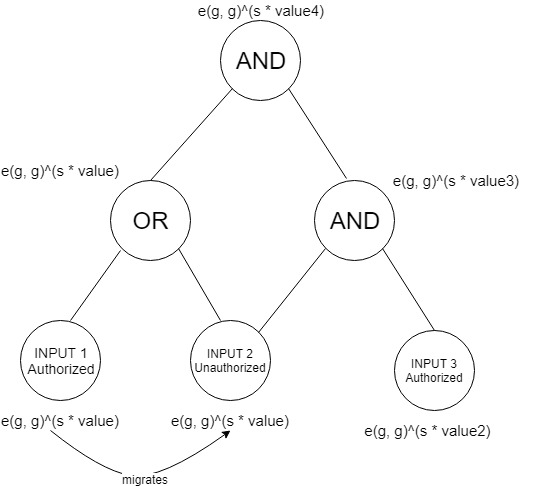
\includegraphics[width=\textwidth,height=8cm,keepaspectratio=true]{figures/BacktrackingAttack.jpg}
\caption{
    The backtracking attack. \cite{gghsw}
}
\end{figure}
\end{center}

\subsubsection{Solutions}

The current solutions that thwart the \textit{Backtracking attack} are based on \textit{multilinear maps} and by using explicit \textit{Fan-Out} gates. 

The solution based on leveled multilinear maps was proposed in \cite{gghsw} that uses a $k + 1$(where $k$ is the depth of the boolean circuit) multiplicative cyclic groups of prime order $p$ $G_1, G_2, ... G_k, G_{k+1}$ and bilinear maps over these groups in order to generate the attribute secrets and the decryption key from a level of the boolean circuit to another. This way the \textit{backtracking attack} is not possible but it is proves to be difficult to implement this since the current implementations of the multilinear maps are not secure. 

The other solution proposed in \cite{fltccd} uses explicit \textit{Fan-Out} gates that have at least one output wire and exactly one input wire. In the proposed schema the \textit{sharing} procedure merges the outputs into a list for the input and also uses another additional list that is used in the reconstruction phase in order to build the desired secrets. This construction is a more efficient that the one in \cite{gghsw} if there are no chained \textit{FO} gates in the circuit paths because it uses only one bilinear map, but otherwise the list increase exponentially increasing the complexity of the schema. Also, this schema is more suitable in practice because it uses bilinear maps that can be implemented based on the known schemas and these constructions are known as being safe so far.

\subsection{Adi Shamir's secret sharing algorithm}

The Shamir's secret sharing procedure was proposed first on \cite{shamir}(1979) and is strongly related to the \textit{threshold gates} described above. This schema proposes a way of sharing a secret $S$ using $S_1, S_2, ..., S_n$ pieces of $S$ and sharing them with $n$ entities and allow the secret $S$ to be reconstructed \textit{if and only if} at least $k, k \le n$ entities know their $S_{i_1}, S_{i_2}, ..., S_{i_k}$ pieces of the $S$ secret. 

\subsubsection{Algorithm}

Let $S$ be a number representing secret that has to be shared, $k$ be the number of entities required for the secret reconstruction and $N$ the total number of entities. To divide $S$ into $N$ pieces $S_1, S_2, ..., S_N$ the algorithm picks a random polynomial $p(x) = a_0 + a_1 \cdot x + ... + a_{k - 1} \cdot x^{k - 1}$ of $k - 1$ degree where $a_0$ represents $S$ (notice that $a_1, ..., a_{k - 1}$ must be random generated numbers) and then assign to each $S_i = p(i), \forall i = {1, 2, ... n}$.

In order to reconstruct the secret $S$ one has to know at least $k$ values of this polynomial and apply a interpolation algorithm in order to discover the $p(0)$ value and thus the $S$ value. The correctness comes from the sharing phase where for any $k$ values in a \textit{Euclidian space} there exists a unique polynomial of degree $k - 1$ that is discovered using the interpolation algorithm.

\subsubsection{Lagrange polynomial}

The \textbf{Lagrange polynomial} is used in \textit{computer science} and \textit{numerical analysis} as a interpolation technique that aproximates the lowest degree polynomial that satisfies the constraint that all the given points for interpolation are exactly matched by the output of this polynomial.

\textbf{Algorithm:} given a set of entries $(x_0, y_0),(x_1, y_1), (x_2, y_2), ..., (x_n, y_n) \in \mathbb{R}^2$ the value of the Lagrange polynomial of degree $n$ in $x$ is given by the formula:

$$L^n(x) = \sum_{i = 0}^n(y_i\prod_{j \neq i, j = 0}^n \frac{x - x_j}{x_i - x_j})$$

This method can be used with the $S_{i_1}, S_{i_2}, ..., S_{i_k}$ from the Shamir secret sharing algorithm in order to compute the value $p(0)$ of the random generated polynomial and thus achieving the secret $S$.

\vspace{200mm}

\section{Extension for the KP-ABE schema based on bilinear maps using boolean circuits with threshold gates}

In this section we present an extension to the current \textit{Key-Policy Attribute based encryption} schema proposed in \cite{fltccd} by defining new \textit{share} and \textit{reconstruction} procedures for boolean circuits with \textbf{threshold gates (k, N)}. This extension was mentioned in the \cite{fltccd} paper, it was proved that threshold gates are suited for this schema, but this extension was not formally defined and analysed. Our extension is important because it allows creating access structures more flexible and expressive than the classical boolean circuits with \textit{OR} and \textit{AND} gates. Also, using threshold gates seems to be more natural than using classical gates when designing access structures for access control systems.

This section also details the security proof of our extension and the implementation using \textbf{jPBC} of the \cite{fltccd} schema with our contribution. 

\subsection{Proposed schema}

To define our extension we'll rewrite the schema proposed in \cite{fltccd} paper and adapt it where it is necessary for threshold gates.

\subsubsection{Description}

Let $eval$ be a function that takes as input a set of gate types $T$, a input array corresponding to the gate input, and returns an array of boolean values corresponding to the output values of the gate.

In our construction $T = \{(k, N) \textrm{ threshold gates }, FO \textrm{ gates}\}$ and the $eval$ function over these gates is defined as it follows:

\begin{itemize}
 	\item \textit{threshold gates ($k$, $N$)}: where $N$ is the number of input values $I = I_1, I_2, ...I_n$ of the gate and $k$ the number of inputs that \textbf{must} be evaluated to $true$ in order to evaluate the gate as true. Thus, $eval((k, N) \textrm{ threshold gate }, I) = [true]$ \textit{if and only if} $\exists I_{i_1}, I_{i_2}, ..., I_{i_k} \subseteq I, $ with the property that $\forall j \in {1, 2, ...k}, I_{i_j} = true$. Otherwise, $eval((k, N) \textrm{ threshold gate }, I) = [false]$.

 	\item \textit{Fan-Out (FO) gates}: takes as input a value $I$ ($true$ or $false$) and has $n$ outputs $O = O_1, O_2, ... O_n$. This gate propagates its input to the outputs as follows: $eval(FO, I) = [I, I, ...I]$ ($n$ times) corresponding to the values assigned to the $O$ outputs array.
\end{itemize}

This function can be used to evaluate the boolean circuits value and see if given a set of attributes, the decryptor can obtain the decryption key, but this function is not used in the schema algorithm.

We denote by $wire_{index}$ the wires that connect the gates. These wire indexes are assigned before the decryption phase and comes with the boolean circuit structure. These wires are indexed top-up from left to right for each boolean circuit level.

\paragraph{Schema definition}

\begin{enumerate}
	\item \textit{Setup($\lambda$, n)}: this procedure chooses a parameter $p$ using $\lambda$, $G_1$ and $G_2$ two multiplicative cyclic groups of prime order $p$, $g$ (any element from $G_1$ except zero or one elements) a generator for $G_1$, a bilinear map $e : G_1 \bigtimes G_1 \rightarrow G_2$, $y \in \mathbb{Z}_p$ and for each $i \in {1, 2, ...,n}$ $t_i \in \mathbb{Z}_p$ and outputs the following structures:

	$$PublicParameters = (p, G_1, G_2, g, e, n, e(g, g)^y, \{g^{t_i} | i \in \{1, 2, ..., n\}\})$$

	$$MasterKey = (y, \{t_1, t_2, ..., t_n\})$$

	\item \textit{Encrypt(m, A, PublicParameters)}: this procedure encrypts the message $m$ with attributes $A \in {1, 2, ..., n}$ chooses a random $s \in \mathbb{Z_p}$ and outputs the structure:

	$$EncryptionResult = (A, ciphertext = m \cdot e(g, g)^{ys}, g^s, \{g^{t_i \cdot s} | i \in A\})$$

	\item \textit{KeyGen(C, MasterKey)}: takes as input the boolean circuit $C$ (with $n$ attribute inputs) associated with the user that wants to obtain the decryption key for $m$. The procedure does the following:
		$$(S, P) = Share(y, C)$$
		$$D = (P, \{g^{S(wire_i)[j] / t_i} | i \in \{1, 2, ..., n\} \textrm{ and } j \in \{1, 2, ... |S(i)|\}\})$$

		\begin{itemize}
			\item \textit{Share($y$, $C$)}
			\begin{itemize}
				\item let $M$ = $[unmarked, \forall \textrm{ gate} \in C]$ $\rightarrow$ Mark all the gates as $unmarked$
				\item let $o$ = $C.root()$ $\rightarrow$ Extract the root of the boolean circuit
				\item $S(o) = [y] \rightarrow$ Assign to the root an array with the y value   
				\item \textit{for each gate} $\tau \in C$ (top-down order) do the followings:
				\begin{itemize}
				    \item if $M(\tau) == unmarked$ and $\tau$ is \textbf{threshold gate $(k, m)$} with $w$ output and $m$ inputs $w_1, w_2, ..., w_m$, then $M(\tau) = marked$ and for each $i \in \{1, ...,|S(w)|\}$ do the followings:
				        \begin{enumerate}
				            \item choose uniformly random $a_1, a_2, ..., a_{k - 1} \in \mathbb{Z}_p$ and let $p(x) = S(w)[i] + a_1 \cdot x + a_2 \cdot x^2 + ... + a_{k-1} \cdot x^{k - 1}$ the associated polynomial from the \textit{Shamir's secret sharing} procedure
				            \item $S(w_q).append(p(q))$ for all $q \in {1, 2, ...m}$  
				        \end{enumerate}
				    \item if $M(\tau) == unmarked$ and $\tau$ is $FO$ gate with input $w$ and $m$ outputs $w_1, w_2, ..., w_m$ then $M(\tau) = marked$ and for each $i \in \{1, 2, ..., m\}$ do the followings:
				    \begin{itemize}
				        \item for each $k \in \{1, ..., |S(w_i)|\}$ do the followings:
				        \begin{enumerate}
				            \item choose uniformly random $a_k \in \mathbb{Z}_p$ and compute $b_k \ \in \mathbb{Z}_p$ such that $(a_k + b_k) \textrm{ mod } p = S(w_i)[k]$
				            \item append $a_k$ to $S(w)$
				            \item append $g^{b_k}$ to $P(w_k)$
				        \end{enumerate}
				    \end{itemize}
				    
				\end{itemize} 
			\end{itemize}
		\end{itemize}
	\item \textit{Decrypt(EncryptionResult, D)}: takes as input the \textit{encryption} result and the \textit{key generation} result and  for $i \in {1, 2, ...,n}$ and $j \in {1, 2, ..., |S(wire_i)|}$ does the following:
        \[   
        V_A(i,j) = 
             \begin{cases}
               e(g^{t_i\cdots}, g^{S(wire_i)[j] / t_i}) = e(g, g) ^{ S(wire_i)[j]\cdots}  &\quad\text{if } i \in A\\
               \text{null,} &\quad \text{if } i \in U \setminus A \\
             \end{cases}
        \]

        $$R = Reconstruct(C, P, V_A, g^s)$$
        $$m = ciphertext / R(o)[1] \textrm{ where o is the root of the circuit }$$
        
		\begin{itemize}
			\item $Reconstruct(C, P, V_A, g^s)$
			\begin{itemize}
				\item let $M$ = $[unmarked, \forall \textrm{ gate} \in C]$ $\rightarrow$ Mark all the gates as $unmarked$
				\item $R(i) = V_A(i)$ for $i \in \{1, 2, ...n\}$
				\item \textit{for each gate} $\tau \in C$ (bottom-up order) do the followings:
				\begin{itemize}
				    \item if $M(\tau) == unmarked$ and $\tau$ is \textbf{threshold gate $(k, m)$} with $w$ output and $m$ inputs $w_1, w_2, ..., w_m$, assert that $|R(w_1)| = |R(w_2)| = ... = |R(w_m)|$ and let $len = |R(w_1)|$, $M(\tau) = marked$ and for each $i \in \{1, ..., len\}$ do the followings:
				    \begin{enumerate}
				        \item choose randomly $B_{i_1}, ..., B_{i_k}$ values from 
				        
				        $R(w_1)[i], R(w_2)[i], ..., R(w_m)[i]$, such that $B_{i_j} != null, \forall j \in \{1, ..., k\}$ and $i_1, ..., i_k$ represent the indexes of the non-null value gates; if the choosing fails (not enough non-null values) $R(w)[i] = null$ and continue with another $i$
				        \item compute for all $j \in \{1, ..., k\}$: $$L(j) = \prod_{jj \neq j, jj = 1}^{k}(\frac{0 - i_{jj}}{i_j - i_{jj}})$$ 
				        \item $$R_w = \prod_{j = 1}^{k} (B_{i_j} ^{L(j)})$$
				        \item $R(w).append(R_w)$
				    \end{enumerate}
				    \item if $M(\tau) == unmarked$ and $\tau$ is \textbf{Fan-Out} gate with input $w$ and $m$ outputs $w_1, w_2, ..., w_m$ then $M(\tau) = marked$ and do the followings:
				    \begin{enumerate}
				        \item split $R(w)$ into  $m$ lists $R_{w_1}, ...,R_{w_m}$ such that $|R_{wire_i}| = |P(wire_i)|, i \in {1, 2, ..., m}$
				        \item $R(w_i).append(R_{w_i}[j] \cdot e(P(w_i)[j], g^s)), i \in \{1, 2, ..., m\}, j \in \{1, 2, ...,|R_{w_i}|\}$ 
				    \end{enumerate}
				\end{itemize}
			\end{itemize}
		\end{itemize}
\end{enumerate}

\subsubsection{Correctness}

\begin{theorem}
The \textit{Key-Policy Attribute based Encryption} scheme proposed above with the extension of threshold gates over boolean circuits satisfies the correctness property.
\end{theorem}

In this paper we'll discuss the correctness of our extension with \textit{threshold} gates over the schema in \cite{fltccd} assuming that the whole schema was already proven as being correct. Thus, in this section we'll prove that given a threshold gate $(k, N)$ and a input value representing the key, this value can be divided to secrets using the \textit{share} procedure and then reconstructed with the \textit{reconstruction} procedure \textit{if and only if} the decryptor has at least $k$ of these shares.

To keep things simple, we'll consider that these gates work only with values (not lists like it is in the actual extension), since in our extension we only iterate through the gate's output list and apply the below approach.

\begin{proof}

Let $e(g, g)^{s \cdot X}$ be the value that represents the key that has to be exchanged, and $\tau = (k, N)$ the threshold gate with one output wire $w$ and $n$ input wires $w_1, w_2, ...,w_n$.

The \textit{share} procedure chooses a random polynomial $P(x) = X + a_1 \cdot x + a_2 \cdot x + ... + a_{k - 1} \cdot x^{k - 1}$ and assigns to the input values of $\tau$ the values $P(1), P(2), ..., P(N)$ as in \textit{Figure 7 }.

\begin{center}
  \begin{figure}[htpb]
\centering
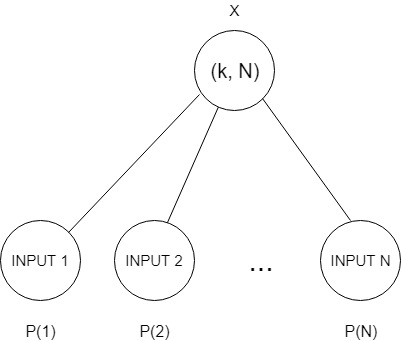
\includegraphics[width=\textwidth,height=5cm,keepaspectratio=true]{figures/shareThreshold.jpg}
\caption{
    The sharing procedure for threshold gates.
}
\end{figure}
\end{center}

In the \textit{reconstruct} phase (see \textit{Figure 8}) the values come as $e(g, g) ^ {s \cdot P(u)}$ or as $null$ for $w_u, \forall u \in \{1, 2, ... N\}$. In this proof we considered the not-null values the first $k$ inputs, but these inputs can have any distribution and also, it is not necessarily that the remaining values are null. After choosing these values (we consider the first K inputs) we can start to create our Lagrange polynomial value. In order to do that, we need firstly to compute $$L(j) = \prod_{jj \neq j, jj = 1}^{k}(\frac{0 - jj}{j - jj}) \textrm{ for all } j \in \{1, ..., k\}$$

After having this we can reconstruct the key:

$$R_w = \prod_{j = 1}^{k} (e(g, g) ^{s \cdot P (j) \cdot L(j)}) \Leftrightarrow$$
$$R_w = e(g, g) ^{\sum_{j = 1}^{k} (s \cdot P (j) \cdot L(j)}) \Leftrightarrow$$
$$R_w = e(g, g) ^{s \cdot \sum_{j = 1}^{k} (P (j) \cdot L(j))} \Leftrightarrow$$
$$R_w = e(g, g) ^{s \cdot P(0)} \Leftrightarrow$$
$$R_w = e(g, g) ^{s \cdot X}$$


\begin{center}
  \begin{figure}[htpb]
\centering
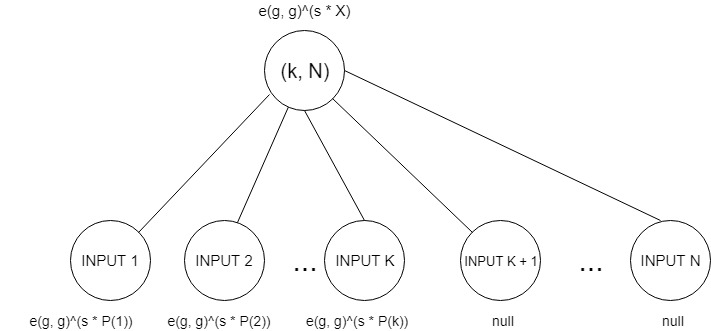
\includegraphics[width=\textwidth,height=5cm,keepaspectratio=true]{figures/reconstructThreshold.jpg}
\caption{
    The reconstruction procedure for threshold gates.
}
\end{figure}
\end{center}

The correctness of the result above comes from the fact that for any $k$ values there exists a unique polynomial of degree $k - 1$ such that all points are part of the polynomial. Since we have these $k$ values and our secret $X$ represents $P(0)$, we can easily compute the Lagrange polynomial value for $0$ and thus obtain the  $X$.

It remains to see what happens if the decryptor doesn't have all the $k - 1$ values: in this case if he gives different values to the \textit{reconstruction} phase, the $P(0)$ will be also different because, as mentioned above, this polynomial is unique. This statement is important because it proves that the construction is also \textbf{collision resistant}.

\end{proof}

\subsubsection{Complexity Analysis}

It is obvious (the complexities come from the \textit{Shamir's secret procedure}) that the complexity of the \textit{threshold gates} for \textbf{share} and \textbf{reconstruct} procedures is based on $k$ and $N$ values, more exactly the first procedure is made in $O(N)$ and the reconstruction in $O(k^ 2)$ (assuming that the choosing of the $k$ values can optimised) for a single key gate output.

The complexity of our extension with \textit{threshold gates}$(k, N)$ is the same if we rewrite the \textit{OR} and \textit{AND} gates with threshold and this is trivial to prove. The tricky part of this section is if we want to write access structures with \textit{threshold gates} with $N > 2$. To compare the complexity of our extension with the schema proposed in \cite{fltccd} we need to rewrite the boolean circuit that has threshold gates with \textit{OR, AND} and \textit{FO} gates. Below we attach some examples of these conversions.

\paragraph{Examples}

In \textit{Figure 9} we can see a conversion of a $(1, 4)$ \textit{threshold gate} to classical \textit{OR} and \textit{AND} gates. Comparing this structure complexity with the \textit{threshold gate} version we can easily notice that the \textit{sharing} procedure for the structure in figure makes more operations than our the threshold gate because the boolean circuit has more nodes. Also, the \textit{reconstruction} phase makes more steps for the same reason.

\begin{center}
  \begin{figure}[htpb]
\centering
\includegraphics[width=\textwidth,height=3cm,keepaspectratio=true]{figures/1-4.jpg}
\caption{
    (1, 4) threshold gate conversion.
}
\end{figure}
\end{center}

In \textit{Figure 10} we can see that we make the same number of steps for the \textit{share} procedure, but for the \textit{reconstruction} procedure is a different story: for the structure in figure, the procedure is done in $k - 1$ steps (the number of internal nodes), but using our structure it increases to $k \cdot (k - 1)$ steps.

\begin{center}
  \begin{figure}[htpb]
\centering
\includegraphics[width=\textwidth,height=3cm,keepaspectratio=true]{figures/4-4.jpg}
\caption{
    (4, 4) threshold gate conversion.
}
\end{figure}
\end{center}

Even though the complexity of the \textit{reconstruct} phase is better for classical gates for the structure in \textit{Figure 10}, in \textit{Figure 11} we can see that using threshold gates the boolean circuit with same semantics is more expressive, but also it is obviously more efficent, because in order to obtain the same semantics, it is needed to use lots of internal gates and also \textbf{Fan-Out} gates that are increase the complexity of the whole structure exponentially.

\begin{center}
  \begin{figure}[htpb]
\centering
\includegraphics[width=\textwidth,height=6cm,keepaspectratio=true]{figures/2-4.jpg}
\caption{
    (2, 4) threshold gate conversion.
}
\end{figure}
\end{center}


\subsection{Security proof}

\begin{theorem}
The \textit{Key-Policy Attribute based Encryption} schema associated proposed in \cite{fltccd} associated with out proposed extension is secure under in the selective model under the decisional bilinear Diffie-Hellman assumption.
\end{theorem}

\begin{proof}

In the \cite{fltccd} paper is described step by step the whole security proof of the schema, in this section we will redefine the \textit{FakeShare} procedure that was defined there with our extension of \textit{threshold gates} without altering the correctness of the proof there and by proving this way that our extension in secure under the \textit{decisional bilinear Diffie-Hellman assumption}.

\paragraph{FakeShare($g^a, C$)}
\begin{itemize}
    \item let $M$ = $[unmarked, \forall \textrm{ gate} \in C]$
	\item let $o$ = $C.root()$
	\item $S(o) = [y] $
	\item \textit{for each gate} $\tau \in C$ (top-down order) do the followings:
    	\begin{itemize}
    	    \item if $M(\tau) == unmarked$ and $\tau$ is \textbf{threshold gate $(k, m)$} with $w$ output and $m$ inputs $w_1, w_2, ..., w_m$, then $M(\tau) = marked$ and for each $i \in \{1, ...,|S(w)|\}$ do the followings:
    	        \begin{enumerate}
    	            \item if $C_w(A) = 1$
    	            \begin{itemize}
    	                \item choose uniformly random $a_1, a_2, ..., a_{k - 1} \in \mathbb{Z}_p$ and let $p(x) = S(w)[i] + a_1 \cdot x + a_2 \cdot x^2 + ... + a_{k-1} \cdot x^{k - 1}$ the associated polynomial from the \textit{Shamir's secret sharing} procedure
    	            \item
                     $\begin{cases}
                       S(w_q).append(p(q)) &\quad\text{if } C_{w_q}(A) = 1\\
                       S(w_q).append(g^{p(q)}) &\quad \text{if } C_{w_q}(A) = 0 \\
                     \end{cases}$
    	            \end{itemize}
    	            
    	            \item if $C_w(A) = 0$
    	            \begin{itemize}
    	                \item choose uniformly random $a_1, a_2, ..., a_{k - 1} \in \mathbb{Z}_p$ and let $p(x) = g^{S(w)[i]} + a_1 \cdot x + a_2 \cdot x^2 + ... + a_{k-1} \cdot x^{k - 1}$ the associated polynomial from the \textit{Shamir's secret sharing} procedure
    	            \item
                     $\begin{cases}
                       S(w_q).append(p(q)) &\quad\text{if } C_{w_q}(A) = 1\\
                       S(w_q).append(g^{p(q)}) &\quad \text{if } C_{w_q}(A) = 0 \\
                     \end{cases}$
    	            \end{itemize}
    	        \end{enumerate}
    	    \item if $M(\tau) == unmarked$ and $\tau$ is $FO$ gate with input $w$ and $m$ outputs $w_1, w_2, ..., w_m$ then $M(\tau) = marked$ do the followings:
    	    \begin{itemize}
    	        \item if $C_w(A) = C_{w_1}(A) = C_{w_2}(A) = ...= C_{w_m}(A) == 1$ then for each $i \in \{1, 2, ..., m\}$ and $j \in \{1, 2, ..., |S(w_i)|\}$:
    	            \begin{enumerate}
    	                \item choose randomly $x_1 \in \mathbb{Z}_p$ and compute $x_2 \in \mathbb{Z}_p$ such that $S(w_i)[j] = (x_1 + x_2)\textrm{mod}p$
    	                \item $S(w).append(x_1)$
    	                \item $P(w).append(g^{x_2})$
    	            \end{enumerate}
    	        \item if $C_w(A) = C_{w_1}(A) = C_{w_2}(A) = ...= C_{w_m}(A) == 0$ then for each $i \in \{1, 2, ..., m\}$ and $j \in \{1, 2, ..., |S(w_i)|\}$:
    	            \begin{enumerate}
    	                \item choose randomly $x_1 \in \mathbb{Z}_p$ and compute $g^{x_2}$ such that $S(w_i)[j] = g^{x_1} * g^{x_2} \Rightarrow g^{x_2} = \frac{S(w_i)[j]}{g^{x_1}} $
    	                \item $S(w).append(g^{x_1})$
    	                \item $P(w).append(g^{x_2})$
    	            \end{enumerate}
    	    \end{itemize}
    	\end{itemize} 
\end{itemize}


\end{proof}

\subsection{Implementation}

In this section we'll discuss the first implementation for the schema proposed in \cite{fltccd} and for our extension with \textit{threshold gates}. We won't get into too much detail here, we'll try to get the core of the implementation here and explain it. Mainly, we'll focus on the way that the proposed schema is translated into \textit{Java} code using the \textbf{jPBC} library. To get brief overview of our classes structure, we used and extended the standard structure for \textit{asymmetric encryption} that is currently implemented in the \textbf{Bouncy Castle} library. Also we used the \textit{Google Guava Library} for different operations on lists and data structures.

\subsubsection{Setup}

The \textbf{Setup} phase creates the \textit{PublicKey Parameters} and the \textit{MasterSecretKey Parameters} that are later used for the \textit{encryption} and \textit{decryption} phases. It uses the \textit{SecureRandom} class proposed by \textbf{Bouncy Castle} library in order generate cryptographic random numbers.

First of all we have to define the bilinear map we're using. For this we already detailed the way of generating these structures in the \textbf{Bilinear maps} so we won't get into details here. In the final implementation we used a \textit{TypeACurveGenerator} with $160$ rBits and $512$ qBits. 

\begin{lstlisting}
pairing = PairingFactory.getPairing(new TypeACurveGenerator(rBits, qBits)
			  .generate())
\end{lstlisting} 

The structure of the output of this method is classical so we'll use the \textit{AsymmetricCipherKeyPair} class for this purpose, where we define the following:

\paragraph{PublicKey Parameters}

$$PublicParameters = (p, G_1, G_2, g, e, n, Y = e(g, g)^y, \{T_i = g^{t_i} | i \in \{1, 2, ..., n\}\})$$

\begin{lstlisting}

p = pairing.getDegree();
G_1 = pairing.getG1();
G_2 = pairing.getG2();
// we can return any element since we have a cyclic multiplicative group
g = pairing.getG1().newRandomElement().getImmutable();
e = pairing;
n = numberOfAttributes;

y = pairing.getZr().newRandomElement().getImmutable();

capitalY = pairing.pairing(groupGenerator.duplicate(), 
                           groupGenerator.duplicate())
                  .powZn(y);

Element[] ts = new Element[n];
for(int i = 0; i < ts.length; ++i) {
    ts[i] = pairing.getZr().newRandomElement();
}

Element[] capitalTs = new Element[n];
for(int i = 0; i < ts.length; ++i) {
    capitalTs[i] = groupGenerator.duplicate().powZn(ts[i]);
}
\end{lstlisting}

\paragraph{MasterSecretKey Parameters}

$$MasterKey = (y, \{t_1, t_2, ..., t_n\})$$

\begin{lstlisting}
y = pairing.getZr().newRandomElement().getImmutable();

Element[] ts = new Element[n];
for(int i = 0; i < ts.length; ++i) {
    ts[i] = pairing.getZr().newRandomElement();
}
\end{lstlisting}

We then encapsulate the above parameters in a \textit{AsymmetricCipherKeyPair} object and return it.


\subsubsection{Encryption}

In this phase takes part the actual encryption of the message. We give as input the message $m$, the attributes used for encryption $A$ and the $PublicParameters$ computed above and it will return the following tuple:

$$EncryptionResult = (A, ciphertext = m \cdot e(g, g)^{ys}, g^s, \{E_i = g^{t_i \cdot s} | i \in A\})$$

\begin{lstlisting}
// choose randomly s
s = publicKey.getPairing()
             .getZr()
             .newRandomElement()
             .getImmutable();

// The assignment is a string of length n 
// with 0 for attribute indexes that are not used for encryption
// and 1 for attribute indexes that are used for encryption
for(int i = 0; i < n; ++i) {
    if (assignment.charAt(i) == '1') {
        e.add(publicKey.getCapitalTAt(i).powZn(s));
    } else {
        e.add(null);
    }
}

// compute e(g, g)^{y * s} 
Element ys = encKey.getPublicKey().getY().duplicate().powZn(s);

encryptionResult.setE(e);
encryptionResult.setCipherText(plaintext.mul(ys));
encryptionResult.setGs(publicKey.getGroupGenerator().duplicate().powZn(s));
encryptionResult.setA(assignment);
\end{lstlisting}

\subsubsection{Key Generation}

This is the phase where the decryption of the the message begins. In a access control system, a user comes with the $MasterKey$ that he knows from the $Setup$ phase and he takes his access structure defined by the boolean circuit he owns (he may have more than one in some systems) and then uses the $KeyGeneration$ method to obtain a decryption key $D$ defined as follows:

$$D = (P, D = \{D_i = g^{S(wire_i)[j] / t_i} | i \in \{1, 2, ..., n\} \textrm{ and } j \in \{1, 2, ... |S(i)|\}\})$$
\begin{center}
    where
\end{center}
$$(S, P) = Share(y, C)$$

The \textit{Share} method takes as input the $y$ value defined in the $MasterKey$ and the boolean circuit $C$ given by the user that wants to access the resource and returns two dictionaries $S$ and $P$ that associate for every wire $w \in C$ a value in $\mathbb{Z}_p$, respectively $G_1$.

To define the boolean circuit that the user uses for access the resource we already discussed in the \textbf{Boolean circuits} section where we showed how to define access structures with classical boolean gates, but also with \textit{threshold gates}.

We define below the signature for the constructors used for creating the boolean circuits and their gates.

\begin{itemize}
    \item \textit{DefaultCircuit(int n, int q, DefaultGate[] gates)} where
    \begin{itemize}
        \item $n$ is the number of attributes ($|U|$) that the boolean circuit takes as input
        \item $q$ is the number of internal gates
        \item $gates$ the gate definition of the circuit (see below)
    \end{itemize}
\end{itemize}

\begin{itemize}
    \item \textit{DefaultGate(GateType type, int index, int[] inputs, int k)} where
    \begin{itemize}
        \item $type$ is the enum type of the gate. Possible values: \textit{INPUT}, \textit{AND}, \textit{OR}, \textit{FO}, \textit{KN}
        \item $index$ the index of the gate
        \item $inputs$ a list of in gate indexes that the currently defined gate takes as input
        \item $k$ (\textbf{optional}) value that is used for for specifing the required number of true values for a \textit{threshold gate} in order for the gate to be evaluated as $true$
    \end{itemize}
\end{itemize}

Also when a \textit{boolean circuit} is created we call a procedure that labels all the wires of the boolean circuit $C$ with a specific index that is later used for assigning values to a specific wire by the $share$ and $reconstruct$ methods. The indexes are assigned top-down from the left to the right.

The procedure of assigning values to each circuit wire is the following:

\begin{lstlisting}
Arrays.sort(gates, Comparator.comparingInt(DefaultGate::getIndex));
List<DefaultGate> reversedGates = Lists.reverse(gates);
Map<CircuitWire, Integer> wireIndexMapping = Maps.newHashMap();

int currentIndex = 0;
for (DefaultGate gate : reversedGates) {
    if (gate.getType() == GateType.INPUT) {
        continue;
    }
    for (int i = 0; i < gate.getInputSize(); i++) {
        CircuitWire circuitWire = new CircuitWire();
        circuitWire.setInputGateIndex(gate.getInput(i));
        circuitWire.setOutputGateIndex(gate.getIndex());

        wireIndexMapping.put(circuitWire, currentIndex);

        currentIndex++;
    }
}
\end{lstlisting}

Then we define a method $getWireIndex$ that takes as input two index wires, the first one representing the input gate and the second one the output gate and returns the index of the wire specified by those gates. 

We can define now the $Share$ procedure:

\begin{lstlisting}
// Parse the gates in top-down order
List<DefaultGate> topDownGates = reverse(circuit.iterator());
for (DefaultGate gate : topDownGates) {
  switch (gate.getType()) {
    case OR: {
      // returns the list of elements of the current gate that have to be
      // shared by this procedure
      List<Element> elements = getSimpleGateElements(s, y, topDownGates, gate);
      
      // propagate unchanged the values
      s.put(circuit.getWireIndex(gate.getInput(0), gate.getIndex()), elements);
      s.put(circuit.getWireIndex(gate.getInput(1), gate.getIndex()), elements);

      break;
    }
    case AND: {
      // returns the list of elements of the current gate that have to be
      // shared by this procedure
      List<Element> elements = getSimpleGateElements(s, y, topDownGates, gate);

      List<Element> l1 = Lists.newArrayList();
      List<Element> l2 = Lists.newArrayList();
        
      // for each element of the wire list
      for (Element element : elements) {
        // choose randomly x1
        Element x1 = pairing.getZr()
            .newRandomElement();
            
        // pick x2 such that element = (x1 + x2) mod p
        Element x2 = pairing.getZr()
                            .newElement(
                                x1.duplicate()
                                  .toBigInteger()
                                  .negate()
                                  .add(element.toBigInteger())
                                );

        l1.add(x1);
        l2.add(x2);
      }

      s.put(circuit.getWireIndex(gate.getInput(0), gate.getIndex()), l1);
      s.put(circuit.getWireIndex(gate.getInput(1), gate.getIndex()), l2);

      break;
    }
    case FO: {
      // returns the list of elements of the FO gate that have to be
      // shared by this procedure associated with each input gate
      Map<Integer, List<Element>> elements = 
            getFOGateElements(s, y, topDownGates, gate);
      List<Element> sElements = Lists.newArrayList();

      // for each input wire of the FO gate
      for (Entry<Integer, List<Element>> entry : elements.entrySet()) {
        List<Element> pElements = Lists.newArrayList();
        
        // for each element of the wire output list
        for (Element element : entry.getValue()) {
          // choose randomly x1
          Element x1 = pairing.getZr()
              .newRandomElement();
          // pick x2 such that element = (x1 + x2) mod p
          Element x2 = pairing.getZr()
              .newElement(
                x1.duplicate()
                  .toBigInteger()
                  .negate()
                  .add(element.toBigInteger())
                );

          sElements.add(x1);
          pElements.add(
                    publicKeyParameters.getGroupGenerator()
                                       .duplicate()
                                       .powZn(x2)
                    );
        }
        // assign to each output wires the p values
        p.put(entry.getKey(), pElements);
      }

      // assign to the input wire the shares
      s.put(circuit.getWireIndex(gate.getInput(0), gate.getIndex()), sElements);

      break;
    }
    case KN: {
      // returns the list of elements of the current gate that have to be
      // shared by this procedure
      List<Element> elements = getSimpleGateElements(s, y, topDownGates, gate);

      // initilize with empty lists the input wires shares
      for (int i = 0; i < gate.getInputSize(); i++) {
        s.put(circuit.getWireIndex(gate.getInput(i), gate.getIndex()), 
              Lists.newArrayList());
      }

      for (Element element : elements) {
        // generate polynomial of K degree
        // The polynomial has the following form: 
        // P(x) = a0 + a_1 * x + ... + a_(k-1) * x^(k-1)
        final List<Element> polynomial = Lists.newArrayList();
        IntStream.range(0, gate.getK())
            .forEach(
              value -> polynomial.add(pairing.getZr().newRandomElement())
            );
        polynomial.set(0, element);
        
        // we create the values that have to be shared:
        // P(1), P(2), ... P(n)
        List<Element> elements = 
          IntStream.range(1, gate.getInputSize() + 1)
                   .mapToObj(value -> evaluatePolynomial(polynomial, value))
                   .collect(Collectors.toList());

        // we add the coresponding share to the input wires:
        // for wire_j => P(j), for each j from 1 to n
        for (int j = 0; j < gate.getInputSize(); j++) {
          s.get(circuit.getWireIndex(gate.getInput(j), gate.getIndex()))
           .add(elements.get(j));
        }
      }

      break;
    }
    case INPUT: {

      break;
    }
    default: break;
  }
}
\end{lstlisting}

The remaining methods that were not defined here are methods that can be implemented different than we did here. To be more specific, the methods $getSimpleGateElements$ or $getFOGateElements$ can be implemented brute-force by traversing the tree or more efficiently by passing the output gates also to each gate. Also, the $evaluatePolynomial$ method can be implemented at least using two ways: first one the classical method where the operations are simply evaluated and a more clever way using the \textit{Horner schema} in order to have a more numerical stability and efficiency.

After having the \textit{share} procedure we can compute the output of the \textit{KeyGeneration} phase:

\begin{lstlisting}

// compute the decryption key
Map<Integer, List<Element>> d = Maps.newHashMap();
for (int i = 0; i < circuit.getN(); i++) {
  d.put(i, Lists.newArrayList());
  List<Element> elements = 
        getSimpleGateElements(s, y, topDownGates, circuit.getGateAt(i));
  
  for (Element element : elements) {
      Element dElement = params.getPublicKeyParameters()
                               .getGroupGenerator()
                               .duplicate()
                               .powZn(
                                  element.div(
                                    params.getMasterSecretKeyParameters()
                                    .getTAt(i)
                                  )
                                );

        d.get(i).add(dElement);
    }
}

return p, d;
\end{lstlisting}

\subsubsection{Decryption}

This method returns the \textit{decryption key} from the encrypted one. It takes as input the $EncryptionResult$ and the shares given by the \textit{share} procedure. 

\begin{lstlisting}
Map<Integer, List<Element>> r = Maps.newHashMap();

// traverse the boolean circuit bottom-up
List<DefaultGate> bottomUpGates = newArrayList(circuit.iterator());
for (DefaultGate gate : bottomUpGates) {
  switch (gate.getType()) {
    case INPUT: {
      // assign to each wire that connects to an input gate the v_A value
      // find the gates that are connected with current gate
      for (DefaultGate outputGate : bottomUpGates) {
        if (outputGate.getType() == INPUT) {
          continue;
        }
        for (int i = 0; i < outputGate.getInputSize(); i++) {
          if (outputGate.getInput(i) == gate.getIndex()) {
            r.put(
              circuit.getWireIndex(gate.getIndex(), outputGate.getIndex()), 
              vA.get(gate.getIndex())
            );
          }
        }
      }

      break;
    }
    case OR: {
      // get the index of the output gate that connects with the gate
      int outputGateIndex = getOutputGateIndex(bottomUpGates, gate);

      List<Element> elements = Lists.newArrayList();
      List<Element> elements1 = r.get(circuit.getWireIndex(gate.getInput(0), 
                                      gate.getIndex()));
      List<Element> elements2 = r.get(circuit.getWireIndex(gate.getInput(1), 
                                      gate.getIndex()));
      for (int i = 0; i < elements1.size(); i++) {
        // choose one of the values that is not null 
        // or null if both of the are null
        if (elements1.get(i) == null) {
          if (elements2.get(i) == null) {
            elements.add(null);
          } else {
            elements.add(elements2.get(i).duplicate());
          }
        } else {
          elements.add(elements1.get(i).duplicate());
        }
      }

      // if this is a final gate, then return the decryption key
      if (outputGateIndex == -1) {
        return elements.get(0);
      }
      r.put(circuit.getWireIndex(gate.getIndex(), outputGateIndex), elements);

      break;
    }
    case AND: {
      // get the index of the output gate that connects with the gate
      int outputGateIndex = getOutputGateIndex(bottomUpGates, gate);
        
      List<Element> elements = Lists.newArrayList();
      List<Element> elements1 = r.get(circuit.getWireIndex(gate.getInput(0), 
                                      gate.getIndex()));
      List<Element> elements2 = r.get(circuit.getWireIndex(gate.getInput(1), 
                                      gate.getIndex()));
      // traverse the list of elements
      for (int i = 0; i < elements1.size(); i++) {
        // if one of the inputs is null, then reconstruct null
        if (elements1.get(i) == null ||
                elements2.get(i) == null) {
            elements.add(null);
        } else {
            // otherwise add the product of the elements
            Element element1 = elements1.get(i).duplicate();
            Element element2 = elements2.get(i).duplicate();
    
            elements.add(element1.mul(element2));
        }
      }
    
      // if this is a final gate, then return the decryption key
      if (outputGateIndex == -1) {
        return elements.get(0);
      }
    
      r.put(
        circuit.getWireIndex(gate.getIndex(), outputGateIndex), 
        elements
      );
    
      break;
    }
    case FO: {
      // get the list of indexes of the output gates that 
      // connect with the current gate
      List<Integer> foGateIndexes = getFOGateIndexes(bottomUpGates, gate);

      // list splitting based on the P map
      Map<Integer, List<Element>> splitRs = Maps.newHashMap();
      // the input wire Rs
      List<Element> gateRs = 
        r.get(circuit.getWireIndex(gate.getInput(0), gate.getIndex()));
      for (Integer foGateIndex : foGateIndexes) {
        int wireIndex = circuit.getWireIndex(gate.getIndex(), foGateIndex);
        int listSize = secretKey.getPElementsAt(wireIndex).size();

        splitRs.put(wireIndex, gateRs.subList(0, listSize));
        gateRs = gateRs.subList(listSize, gateRs.size());
      }

      // for each gate that has as input the current gate
      for (Integer foGateIndex : foGateIndexes) {
        // determine the wire index determined by the current gate
        // and the gate that has as input the current gate
        int wireIndex = circuit.getWireIndex(gate.getIndex(), foGateIndex);
        
        // compute the values reconstructed for this wire
        List<Element> elements = Lists.newArrayList();
        for (int j = 0; j < splitRs.get(wireIndex).size(); j++) {
          // propagate null if the the shared value is null
          if (splitRs.get(wireIndex).get(j) == null) {
            elements.add(null);
            continue;
          }
          // multiplication of the value shared with the 
          // pairing of the associated P value and g^s
          Element element = splitRs.get(wireIndex)
                                   .get(j)
                                   .duplicate()
                                   .mul(
                                      pairing.pairing(
                                        secretKey.getPElementsAt(wireIndex)
                                                 .get(j), 
                                        gs
                                      )
                                    );
         
          elements.add(element);
        }
        // add the reconstructed values to the wire
        r.put(wireIndex, elements);
      }

      break;
    }
    case KN: {
      // get the index of the output gate that connects with the gate
      int outputGateIndex = getOutputGateIndex(bottomUpGates, gate);

      // get the size of the shared lists
      // notice that the list sizes must be equal
      int size = -1;
      for (int i = 0; i < gate.getInputSize(); i++) {
        if (size == -1) {
          size = r.get(circuit.getWireIndex(gate.getInput(i), gate.getIndex()))
                  .size();
        }
      }

      // initilize the output wire of the current gate with empty list
      r.put(
        circuit.getWireIndex(gate.getIndex(), outputGateIndex), 
        Lists.newArrayList()
      );
      
      for (int i = 0; i < size; i++) {
        Element element;
        List<Integer> ks = Lists.newArrayList();
        List<Element> elements = Lists.newArrayList();
        // choose the first k elements from inputs that are not null
        for (int j = 0; j < gate.getInputSize(); j++) {
          List<Element> rElements = 
            r.get(circuit.getWireIndex(
              gate.getInputIndexAt(j), 
              gate.getIndex()
              )
            );
          if (rElements.get(i) == null || ks.size() >= gate.getK()) {
			continue;
		  }

          ks.add(j + 1);
          elements.add(rElements.get(i));
        }

        // for each of these k values
        for (int j = 0; j < ks.size(); j++) {
          // compute the product value from the Lagrange polynomial
          // associated with each P(ks[j]) value
          element = pairing.getZr().newOneElement();
          Element xjElement = pairing.getZr().newElement(ks.get(j));

          for (int jj = 0; jj < gate.getK(); jj++) {
            if (jj == j) {
              continue;
            }

            Element zeroElement = pairing.getZr().newZeroElement();
            Element xjjElement = pairing.getZr().newElement(ks.get(jj));

            element.mul(zeroElement.duplicate()
                .sub(xjjElement)
                .div(xjElement.duplicate().sub(xjjElement))
            );
          }

          elements.get(j).powZn(element);
        }

        // multiplication of all the inputs that results
        // to the reconstruction of the P(0) Lagrange
        // polynomial value
        element = elements.get(0);
        for (int j = 1; j < gate.getK(); j++) {
          element = element.mul(elements.get(j));
        }

        // assign the obtained value to that wire
        r.get(circuit.getWireIndex(gate.getIndex(), outputGateIndex))
         .add(element);
      }

      break;
    }
    default:
      break;
  }

\end{lstlisting}

\subsection{Applications}

\section{Conclusions}

\pagebreak

\blankpage

\begin{thebibliography}{9}

\bibitem{fltccd} 
Ferucio Laurențiu Țiplea, Constantin Cătălin Drăgan, 
\textit{Key-policy Attribute-based Encryption for Boolean Circuits from Bilinear Maps}, 2014.

\bibitem{gghsw} 
Sanjam Garg, Craig Gentry, Shai Halevi, Amit Sahai, Brent Waters 
\textit{Attribute-Based Encryption for Circuits from Multilinear Maps}, 2013
 
\bibitem{gpsw} 
Vipul Goyal, Omkant Pandey, Amit Sahai, Brent Waters 
\textit{Attribute-Based Encryption for Fine-Grained Access Control of Encrypted Data}, 2006

\bibitem{ggh}
Sanjam Garg, Craig Gentry, Shai Halevi
\textit{Candidate Multilinear Maps from Ideal Lattices}, 2012

\bibitem{msz}
Eric Miles, Amit Sahai, Mark Zhandry
\textit{Annihilation Attacks for Multilinear Maps:Cryptanalysis of Indistinguishability Obfuscation over GGH13}, 2016

\bibitem{shamir}
Adi Shamir
\textit{How to Share a Secret}, 1979

\bibitem{blakley}
G. R. Blakley
\textit{Safeguarding cryptographic keys}, 1899

\bibitem{brickell}
E. F. Brickell
\textit{Some ideal secret sharing schemes. Journal of Combinatorial Mathematics and Combinatorial Computing}, 1989

\bibitem{isn}
M. Ito, A. Saito, and T. Nishizeki
\textit{Secret Sharing Scheme Realizing General Access Structure}, 1987

\bibitem{jpbc}
Angelo {De Caro} and Vincenzo Iovino
\textit{jPBC: Java pairing based cryptography Library}, 2011

\bibitem{pbc}
Ben Lynn
\textit{Pairing based cryptography library}

\bibitem{gmp}
\href{https://gmplib.org/\#WHAT}{https://gmplib.org/\#WHAT}
\textit{The GNU Multiple Precision Arithmetic Library}

\bibitem{bc}
\href{https://www.bouncycastle.org/about.html}{https://www.bouncycastle.org/about.html}
\textit{The Legion of the Bouncy Castle}

\bibitem{gghvv}
Craig Gentry, Sergey Gorbunov, Shai Halevi, Vinod Vaikuntanathan, Dhinakaran Vinayagamurthy
\textit{How to Compress (Reusable) Garbled Circuits}, 2013

\bibitem{shamirid}
Adi Shamir
\textit{Identity-Based Cryptosystems and Signature Schemes}, 1984 

\bibitem{sok}
Sakai R., Ohgishi K., Kasahara M.
\textit{Cryptosystems based on pairings}, 2000 

\bibitem{bf}
Dan Boneh, Matt Franklin
\textit{Identity-based encryption from the Weil pairing}, 2001

\bibitem{ka}
Parmar Vipul Kumar J, RajaniKanth Aluvalu
\textit{Key Policy Attribute Based Encryption (KP-ABE): A Review}, 2015

\bibitem{idwiki}
\href{https://en.wikipedia.org/wiki/ID-based_encryption}{https://en.wikipedia.org/wiki/ID-based\_encryption}

\bibitem{abecryptostack}
\href{https://crypto.stackexchange.com/questions/17893/what-is-attribute-based-encryption?utm_medium=organic&utm_source=google_rich_qa&utm_campaign=google_rich_qa}{https://crypto.stackexchange.com/questions/17893/}

\bibitem{abewiki}
\href{https://en.wikipedia.org/wiki/Attribute-based_encryption}{https://en.wikipedia.org/wiki/Attribute-based\_encryption}

\bibitem{bilinearmapwiki}
\href{https://en.wikipedia.org/wiki/Bilinear_map}{https://en.wikipedia.org/wiki/Bilinear\_map}

\bibitem{dbdhwiki}
\href{https://en.wikipedia.org/wiki/Decisional_Diffie\%E2\%80\%93Hellman_assumption}{https://en.wikipedia.org/wiki/Decisional\_Diffie\%E2\%80\%93Hellman\_assumption}

\bibitem{booleancircuitwiki}
\href{https://en.wikipedia.org/wiki/Boolean_circuit}{https://en.wikipedia.org/wiki/Boolean\_circuit}

\bibitem{shamirwiki}
\href{https://en.wikipedia.org/wiki/Shamir\%27s_Secret_Sharing}{https://en.wikipedia.org/wiki/Shamir\%27s\_Secret\_Sharing}

\bibitem{lagrangewiki}
\href{https://en.wikipedia.org/wiki/Lagrange_polynomial}{https://en.wikipedia.org/wiki/Lagrange\_polynomial}

\end{thebibliography}

\vspace{\baselineskip}

\end{document}
